%Dokumenttyp + Encoding
\documentclass[final, paper=a4, paper=portrait, pagesize=auto, fontsize=10pt,english]{scrartcl}
\usepackage[utf8]{inputenc}

\usepackage[a4paper, total={6.5in, 9in}]{geometry}
\usepackage{graphicx}
\usepackage[]{hyperref}
\usepackage{amsmath}

\usepackage{lmodern} %Schriftarten
\usepackage[english]{babel}
\usepackage{color}
\usepackage{placeins}
\definecolor{mygreen}{rgb}{0.33,0.63,0.33}
\definecolor{mygray}{rgb}{0.95,0.95,0.95}
\definecolor{myblue}{rgb}{0.23,0.23,0.52}
\renewcommand{\arraystretch}{1.5}


\usepackage{listings} %for code
\lstset{ 
	 backgroundcolor=\color{mygray},
	 commentstyle=\color{mygreen},
	 numbers=left,
	 keywordstyle=\textbf,
	 language=C++,
	 tabsize=3,  
	 basicstyle=\footnotesize,
}


\begin{document}

\begin{titlepage}
	\centering
	
\includegraphics[width=0.15\textwidth]{brockLogo}\par\vspace{1cm}
	{\scshape\LARGE Brock University\par}
	\vspace{0.5cm}
	{\Large Department of Computer Science\par}
	\vspace{1cm}
	{\Large Report on the final project of COSC 3P98\par}
	\vspace{1.5cm}
	{\huge\bfseries Mandelbrot and Julia Sets\par}
	\vspace{2cm}
	{\Large\itshape Torben Krüger, Maike Rees\par}
	\vspace{2cm}	
	{\large January 2016\par}
\end{titlepage}

\newpage
 
\section{Introduction}
During the process of the course, fractals catched our interest so we desided to make an application about fractals for our final project of the course. The Mandelbrot Set is one of the most popular fractals and it is closely related to the Julia Set so we chose it as our main focus. There are a lot of android apps, online applications and pretty pictures about and of Mandelbrot Sets that inspired us further more. 

We developed the Application in c/c++ with openGl, freeglut and freeimage. We created it on Windows 7 in Eclipse Mars and migrated it later into a visual studio(2013) project.

\section{Functionality}
The Application demonstrates the relation between the Mandelbrot set and Julia sets. Furthermore you get interesting observations through the coloring of the sets. Additionally, images can be saved.
Here is a screenshot of our program.\\\\
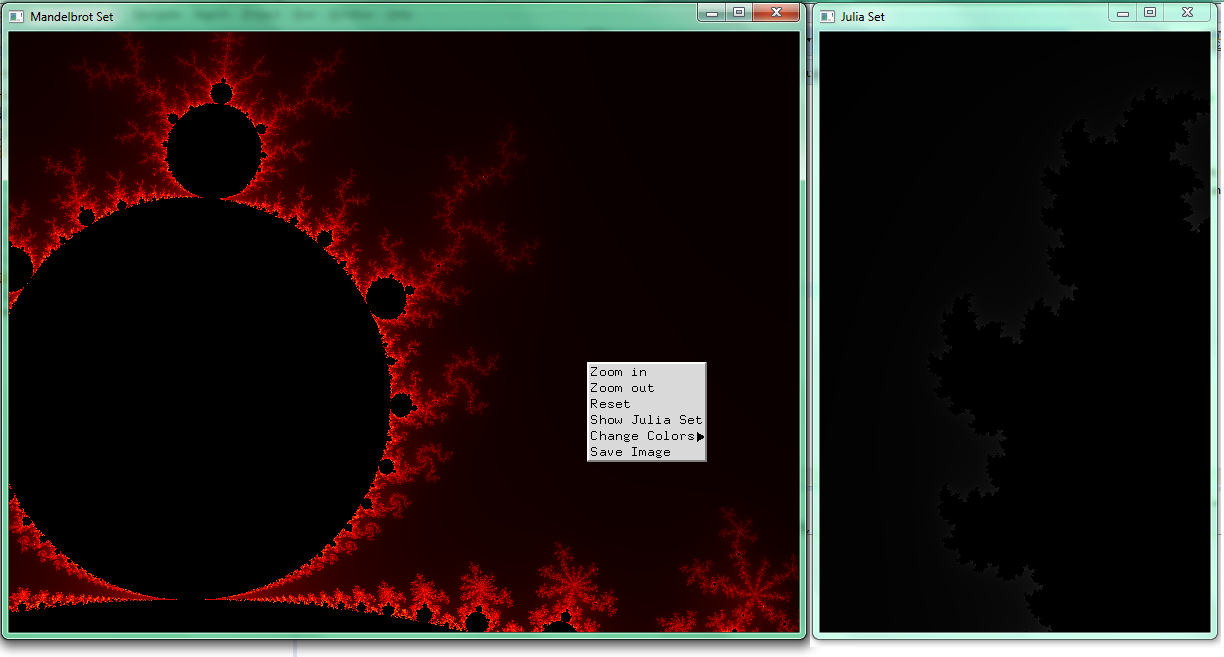
\includegraphics[width=1.0\textwidth]{screenie1}


\section{User Manual}
The Application comes with two windows. One where the Mandelbrot set is shown and in the other one you can see a Julia set. 

You have multiple options here. With left-click of your mouse you can zoom into the chosen set. The point of your mouse click is going to be the center of the zoomed image.

With a right click a context menu opens. You can chose to zoom in and out, reset the set, change the color or save an image of the set. 

If you open this menu in the Mandelbrot set you additionally have the option to show the Julia set of the chosen Point. It will then show the according Julia Set in the second Window.

\section{Architecture and Implementation}
The architecture of the application is not too complicated. It is object-oriented and structured into header and cpp - files.

\subsection{Complex Numbers}
Since we're calculating with complex numbers most of the time in those sets there is a class called Complex.h that describes those complex numbers as a struct. Every complex number comes with a real and imaginary part which are represented by two integers.

This struct also overloads methods for the + and * operator. It also contains a method that squares the number and one that calculates the absolute value of the complex number. Those methods are all needed to calculate the sets.

\begin{lstlisting}
struct complex {
	double r, i;
	double getAbsolute() {...}
	complex pow2() {...}
	inline complex operator+(complex a) {...}
	inline complex operator*(complex a) {...}
};
\end{lstlisting} 

\subsection{Mandelbrot Set}
For a Mandelbrot set we set up a header and the cpp-file that implements the header methods. 
The Mandelbrot set has public methods to calculate the set, zoom in and out of it, reset it as well as some Getters and Setters. 

\begin{lstlisting}
class MandelbrotSet {
public:
	MandelbrotSet(unsigned int, unsigned int);
	virtual ~MandelbrotSet();
	void calculate();
	void setWidth(unsigned int);
	void setHeight(unsigned int);
	void setIterations(unsigned int);
	void reset();
	void zoom(unsigned int, unsigned int);
	void zoomOut(unsigned int, unsigned int);
	void setColorMode(int);
};
\end{lstlisting}

\subsection{Julia Set}
Looking at the formular of both sets, one can see that they are very close. That is why we decided to let the Julia set be a child of the Mandelbrot set. Since there are only a few changes that we had to make in the Julia classes, we save a lot of code and our implementation gets a lot easier with this design decision. 

The Julia set only overrides the cnstructor and the calculate(), draw() and reset() methods. Additionally it has a complex number k, that is needed for the calculation.

\begin{lstlisting}
class JuliaSet: public MandelbrotSet {
public:
	JuliaSet(unsigned int, unsigned int);
	void draw(unsigned int, unsigned int, complex);
	void calculate();
	void reset();
	complex k;
};
\end{lstlisting}

\subsection{The Main Class} 	
The Main.cpp puts it all together. It sets up the OpenGl / freeglut environment, handles mouse event and the menus and starts the drawing of the sets. \\\\
When clicking on an option of the menu the program often needs to know where the mouse is right now to calculate with the right coordinates. For this purpose the application is using the passive motion function that glut offers. It always saves the current mouse coordinates in the global struct.

\section{Coloring}
The Mandelbrot set itself only tells us if the pixel is in the set or not. So basically only two colors are needed to display the Mandelbrot set. Like in this screenshot (chose colormode 'pure' in the application). \\\\
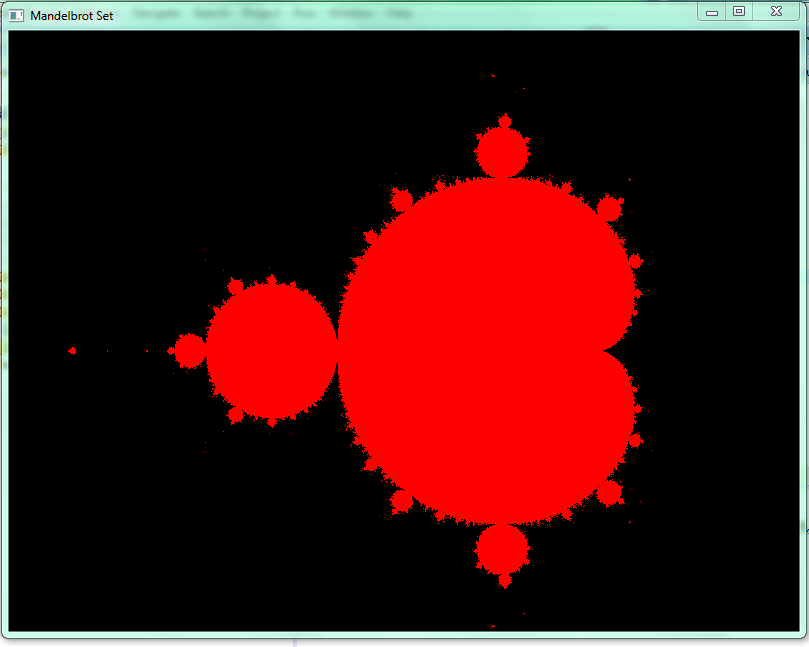
\includegraphics[width=0.7\textwidth]{screeniePure}

A lot of fun comes with different coloring techniques so we want to take a closer look to it.

The Mandelbrot calculates its pixel with a preset maximum number of iterations (because it can calculate infinitely, but thats obviously not helping us). The bigger the maximum number of iterations, the more precise is the image. But this also means that with a big number of max. iterations the calculating time is way longer that with a small number. So the idea behind the iterations is that every iterations looks a little bit closer into the Mandelbrot set. So at some point, the algorithm will determine that a pixel is not included in the mandelbrot set and will then break the for-loop. If the pixel is inlcuded in the Mandelbrot set the for-loop will terminate regularly after all iterations have been run through.\\ \\ 
To make this a little more clear, here is the code snippet:\\

\begin{lstlisting}
void MandelbrotSet::draw(unsigned int x, unsigned int y, complex c) {
	complex z = c;
	unsigned int n = 0;

	for (n = 0; n < iterations; n++) {

		if (z.getAbsolute() > 4) {
			break; // the pixel is not in the Madelbrot set
		}
		z = z.pow2() + c;
	}
	data[x + y * width] = getColor(n); // get the color based on the iteration
}
\end{lstlisting}

This means that every pixel has a number n that is the iteration at wich the for-loop terminated.
For the pixels that are in the Mandelbrot set
\begin{displaymath} 
n = number \: of \: max \: iterations
\end{displaymath}
and for all the others
\begin{displaymath} 
0 \leq n  \: \textless \: number \: of \: max \: iterations
\end{displaymath}

According to this number n the different coloring methods calculate the color.

\subsection{Linear Coloring}
E.g. the greyscale colormode uses a linear coloring method. 
First of all the step between each color is calculated. That means if the number of iterations is big the steps are small and the other way round. Then the red value is calculated. The pixels within the Mandelbrot set get the color black.

\begin{lstlisting}
float step = 1.0f / iterations;
...
// greyscale
red = 2 * n * step * 255;
if (n > iterations - 2) {
	red = 0;
}
blue = red;
green = red;
\end{lstlisting}

In the red and white colormode, the application uses a gradient from black to red for the first half of the iterations and a gradient from red to white for the second half of the iterations.
\begin{lstlisting}
red = 2 * n * step * 255;
if (n < iterations / 2 - 1) { // black to red
	green = 0;
	blue = 0;
} else if (n < iterations - 2) { // red to white
	green = 255;
	blue = 255;
} else { // pixel in the set are black
	red = 0;
	green = 0;
	blue = 0;
}
\end{lstlisting}

\subsection{Logarithmic Coloring} 

The Logarithmic coloring method provides more detailed coloring for the edges of the Mandelbrot set. The linear coloring uses one color gradient wheras the logarithmic coloring uses 7 different color gradients. Furthermore it seperates the iterations in unequal parts to apply the gradient.

\begin{lstlisting}
if (n == iterations) {
} else if (n < 64) {
	red = n * 2.0f;
} else if (n < 128) {
	red = ((((n - 64.0f) * 128.0f) / 126.0f) + 128.0f);
} else if (n < 265) {
	red = ((((n - 128.0f) * 62.0f) / 127.0f) + 193.0f);
} else if (n < 512) {
	red = 1.0f;
	green = ((((n - 256.0f) * 62.0f) / 255.0f) + 1.0f);
} else if (n < 1024) {
	red = 1.0f;
	green = ((((n - 512.0f) * 63.0f) / 511.0f) + 64.0f);
} else if (n < 2048) {
	red = 1.0f;
	green = ((((n - 1024.0f) * 63.0f) / 1023.0f) + 128.0f);
} else /*if (n < 4096)*/ {
	red = 255;
	green = ((((n - 2048.0f) * 63.0f) / 2047.0f) + 192.0f);
}
\end{lstlisting}

The result is that the edges are more nicely shaded in comparison to the linear gradient. As you see in the two images below, the logarithmic gradient has a smooth gradient from red to yellow and the linear gradient 'jumps' between red and white. \\\\

Difference between logarithmic (left) and linear (right) coloring. \\
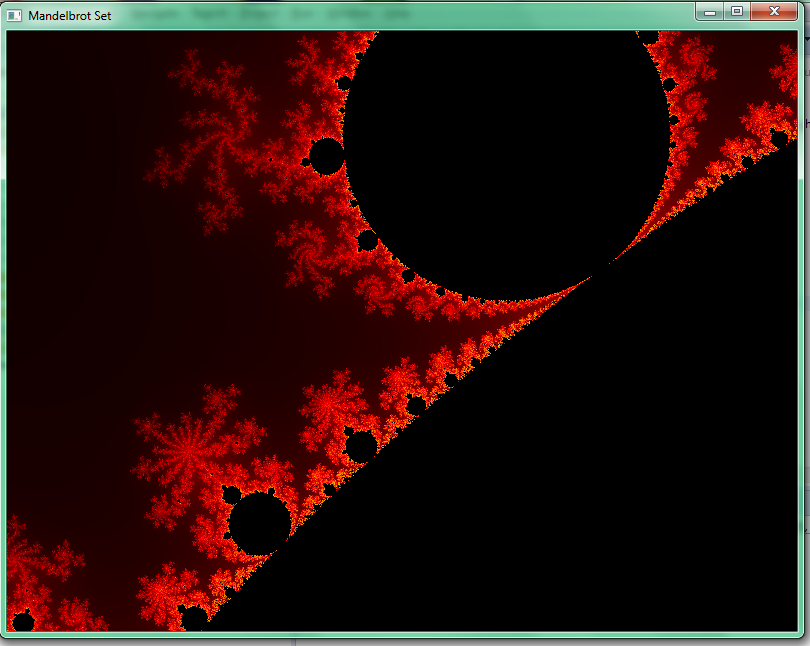
\includegraphics[width=0.5\textwidth]{screenie2}
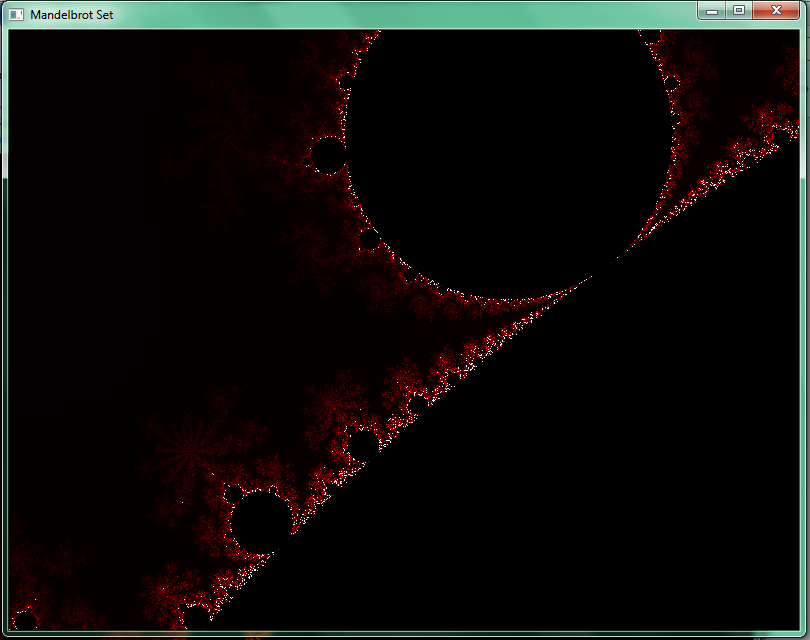
\includegraphics[width=0.5\textwidth]{screenie4}
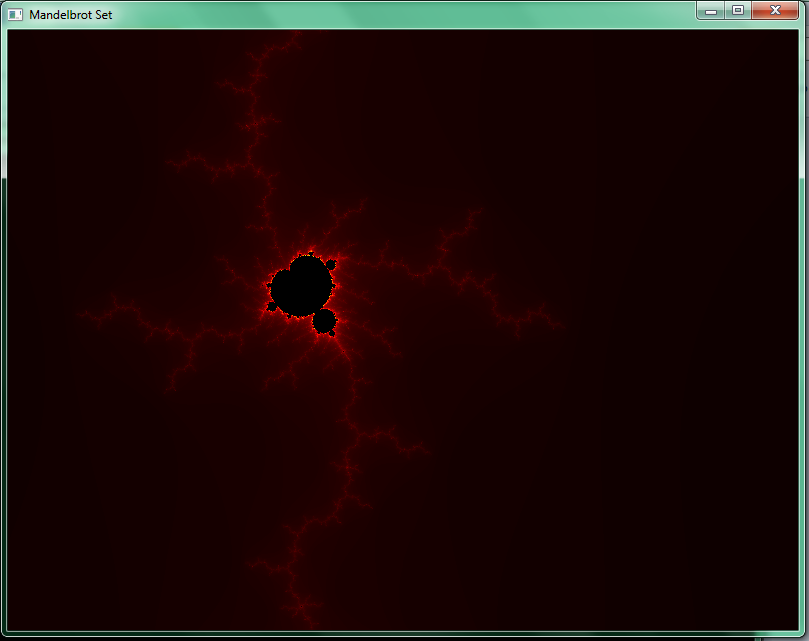
\includegraphics[width=0.5\textwidth]{screenie7}
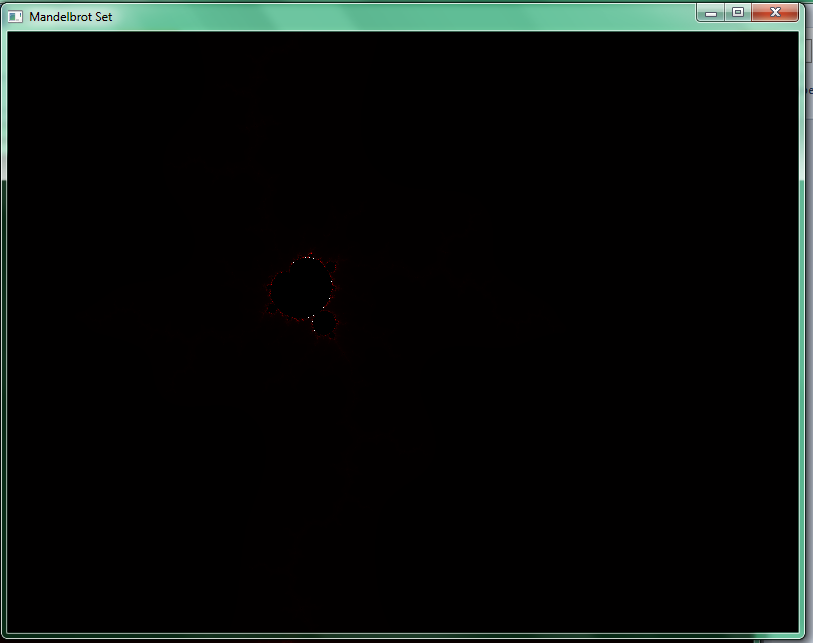
\includegraphics[width=0.5\textwidth]{screenie8}



\section{Mathematic Background}
\section{Discussion}
Including the coloring gives a nice extra observation. Let's discuss this with the help of an example. \\
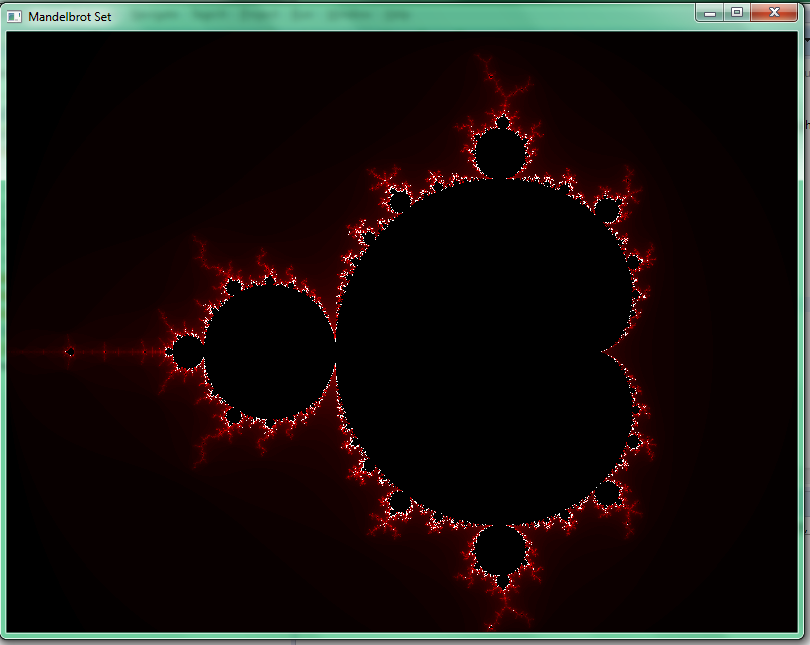
\includegraphics[width=0.7\textwidth]{screenie5}

The Mandelbrot set has the property that the pixels that are closer to the boarder have higher iteration numbers. For this coloring method this means that white pixels are very close to the boarder of the set and red pixel are closer than black pixels but not as close as the white pixels to the boarder. 

This means that the red pixels that look like roots of a tree tell us that there is a boarder some where close to them. So if we zoom in deep enough we will find a part of the Mandelbrot set there as well. \\

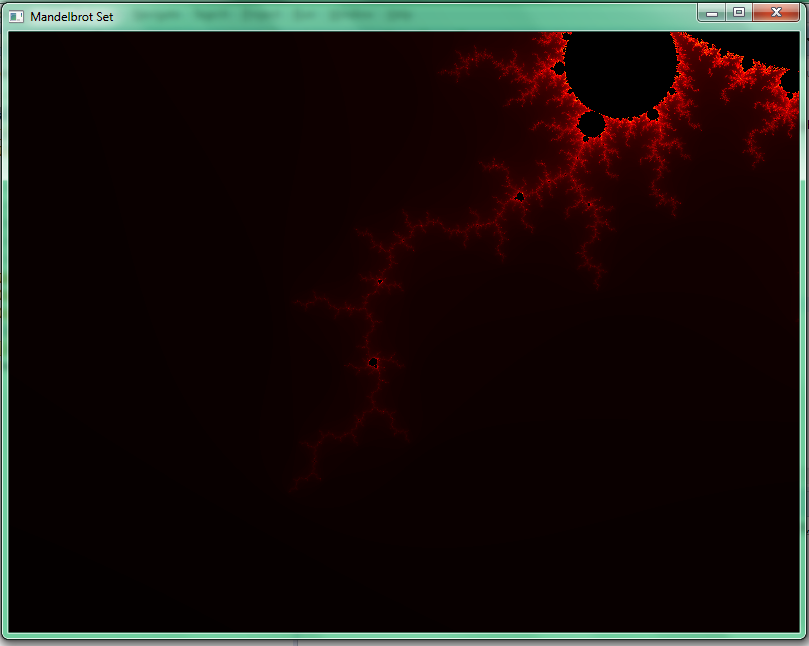
\includegraphics[width=0.4\textwidth]{screenie6}
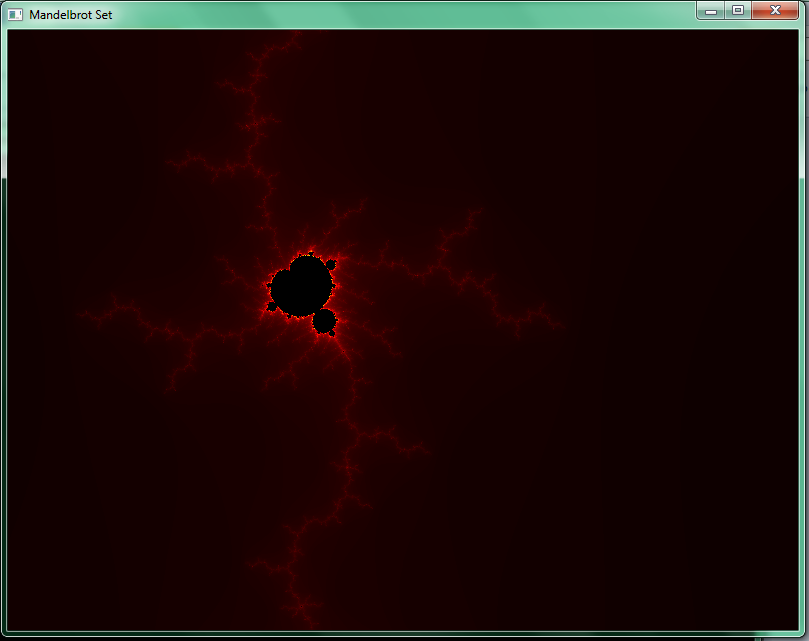
\includegraphics[width=0.4\textwidth]{screenie7}

Looking at these zoomed pictures we also see that the small part of the Mandelbrot set has the same shape as the big one where we started. This is another interesting property of the Mandelbrot set.

\section{References}

\end{document}